\chapter{Hardware Implementation}\label{quantization}
\indo{Short introduction}

\section{Hardware-Aware Optimizations}

\subsection{Tensor Multiplication and Scaling}
Each self-attention head performs two tensor multiplications (referred to as \textit{matmul} blocks in figure \ref{fig:self-attention-multi-head}), which are normally expressed using Einstein Summation notation \cite{59-barr1991einstein}, which is supported by mathematical and machine learning libraries like \texttt{NumPy} or \texttt{PyTorch}. However, not present by default in HLS, it required careful design of the calculation loops in order to not cripple the performance by unnecessary computations and pseudo-random data accesses. As part of this research, an efficient and fully-customizable HLS block has been designed, that uses a very similar interface to the Python equivalent.

\begin{figure}[hpt!]
  \centering
  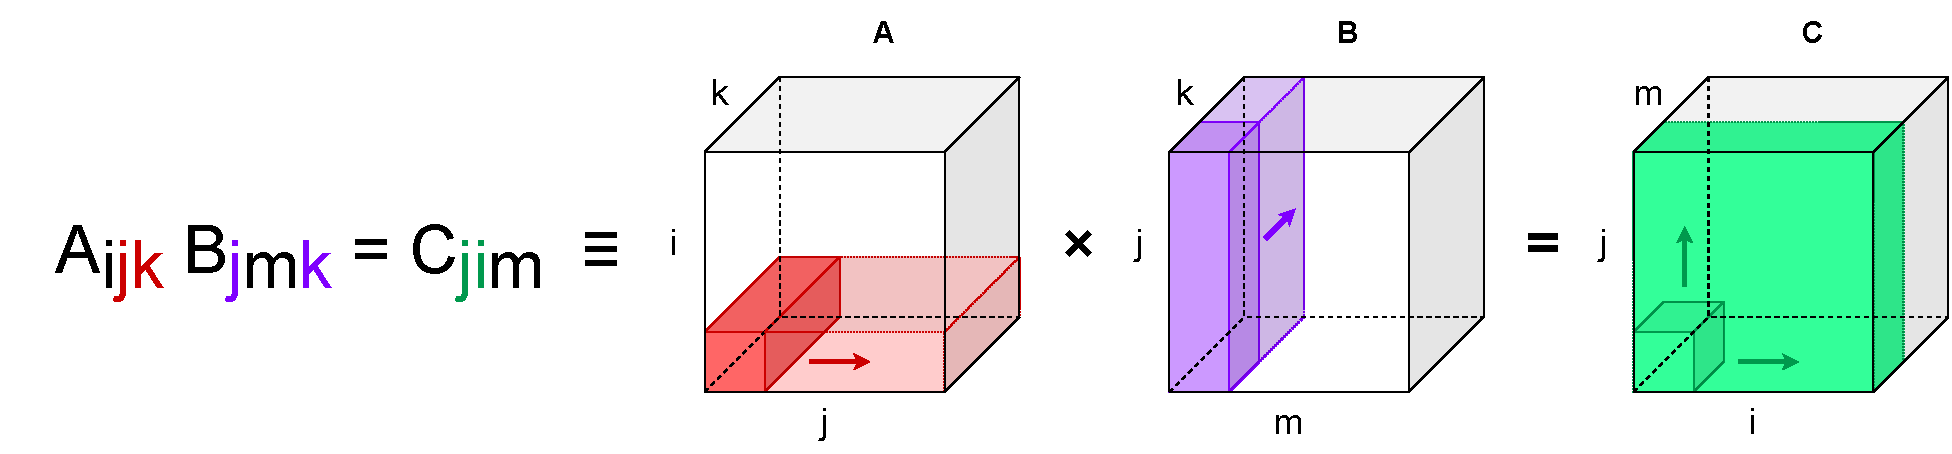
\includegraphics[trim={0cm 0cm 0cm 0cm}, width=0.8\textwidth, center]{models/einsum.pdf}
  \caption{Visualization of a tensor operation expressed in Einstein Summation notation.}
  \label{fig:einsum}
\end{figure}

Figure \ref{fig:einsum} shows a visualization for an example notation to give a better understanding of the necessary flexibility of a formula. The translation between notations using the custom tool is showcased in listing TODO. While the \texttt{PyTorch} implementation uses 4-dimensional tensors, the first dimension refers to the batch, which is not present in the hardware implementation that processes input samples one-by-one.

\todofig{Code listing showing starting \texttt{PyTorch} code and resulting C++ HLS implementation}
\todofig{|}
\todofig{|}
\todofig{|}
\todofig{|}
\todofig{|}

Another simple optimization used alongside the tensor multiplication blocks was the change in size scaling from using division to performing an arithmetic right shift (ASR), which requires precomputing the logarithm of the size, seen in equation \ref{eq:log-div}, vastly simplifying the otherwise computationally expensive hardware required at run-time.

\begin{equation}\label{eq:log-div}
  \frac{x}{\sqrt{\text{size}}} \equiv \text{ASR}(x,\; \log_2 \sqrt{\text{size}}) \equiv \text{ASR}(x,\; \frac{1}{2}\log_2 \text{size})
\end{equation}


\subsection{Softmax and Log Softmax Activation}
Despite an already existing \hlsml implementation of the softmax activation function, computing the logarithm of its result is not as simple as it may seem. This is because the numerical stability and computational efficiency of this operation is often explored in-depth \cite{60-blanchard2019accurate} and varies depending on the programming language and target platform.

\begin{figure}[hpt!]
  \centering
  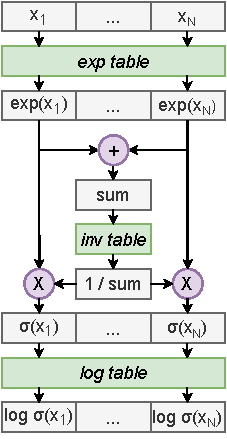
\includegraphics[trim={0cm 0cm 0cm 0cm}, width=0.2\textwidth, center]{models/log_softmax_naive.pdf}
  \caption{Direct hardware implementations of log softmax.}
  \label{fig:log-softmax-naive}
\end{figure}

The naive implementation comes straight from the definition of taking a logarithm of softmax, seen in equation \ref{eq:softmax}, and the required hardware operations are shown in figure \ref{fig:log-softmax-naive}.

\begin{equation} \label{eq:softmax}
    \sigma (x_i) = e^{x_i} / \sum_{j=1}^{N} e^{x_j}
\end{equation}

This report proposes a different way of mapping this operation to hardware to improve stability while shortening the critical path and using less resources. It is based on the derivation shown in equation \ref{eq:log-softmax}.

\begin{equation} \label{eq:log-softmax}
    \log (\sigma (x_i)) = log(e^{x_i} / \sum_{j=1}^{N} e^{x_j}) = \log(e^{x_i}) - \log(\sum_{j=1}^{N} e^{x_j}) = e^{x_i} - \log(\sum_{j=1}^{N} e^{x_j})
\end{equation}

The resulting hardware operations are depicted in figure \ref{fig:log-softmax-opt}. It is important to note, that operations like exponentiation, division or taking a logarithm usually rely on precomputing a wide range of values and mapping them in BRAMs or LUTs to allow for lookup on run-time. Hence, the optimized design requires one less of such lookups while also replacing multiplication by a subtraction, which can be simpler to express in hardware.

\begin{figure}[hpt!]
  \centering
  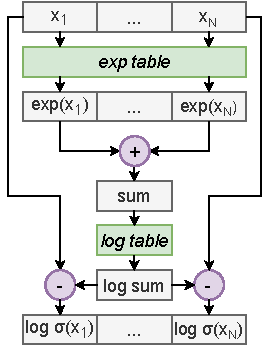
\includegraphics[trim={0cm 0cm 0cm 0cm}, width=0.2\textwidth, center]{models/log_softmax_opt.pdf}
  \caption{Optimized hardware implementations of log softmax.}
  \label{fig:log-softmax-opt}
\end{figure}

Although further simplifications, including approximating the summation by finding the maximum (see equation \ref{eq:log-softmax-max}) or simply omitting the logarithm portion of the expression, were also explored, they noticeably lowered the final accuracy and were thus abandoned.

\begin{equation} \label{eq:log-softmax-max}
    \log (\sigma (x_i)) = e^{x_i} - \log(\sum_{j=1}^{N} e^{x_j}) = e^{x_i} - \sum_{j=1}^{N} \log(e^{x_j}) = e^{x_i} - \sum_{j=1}^{N} x_j \approx e^{x_i} - \max(x)
\end{equation}


\section{Analytical Latency and Resource Model}
\indo{Reason about computational complexity, include a diagram of self-attention tensor multiplications based on contents of Deep Learning lectures}
\indo{|}
\indo{|}
\indo{|}
\indo{|}
\indo{|}
\indo{|}
\indo{Derive simple latency and resource (likely only DSP as others are too difficult) model, that will be verified in evaluation chapter}
\indo{|}
\indo{|}
\indo{|}
\indo{|}


\section{Post-training Quantization}
\indo{Explain my custom algorithm and where it draws inspirations}
\indo{Walk through the steps and explain the parameters, pointing to provided algorithm}
\indo{Explain how the very long simulation time prevents more mature solutions like Bayesian Optimization or even Grid Search (this solution already took 120+ hours on a medium-sized design with 60 type parameters)}
\indo{Talk about correlation of neighboring bit widths and how this is exploited (i.e. by resuming with previous width + the whole idea is based on that instead of a full gradient descent style search)}
\indo{|}
\indo{|}
\indo{|}
\indo{|}
\indo{|}
\indo{|}
\indo{|}
\indo{|}
\indo{|}
\indo{|}

\begin{algorithm}
  \caption{Algorithm for performing post-training quantization search}\label{alg:post-training-quant}
  \begin{algorithmic}
  \Function{PostTrainingQuantization}{neg\_accuracy\_tolerance, pos\_accuracy\_tolerance}

  \State $previous\_width \gets null$
  \State $max\_decrement \gets neg\_accuracy\_tolerance \cdot 2$ \Comment{Maximum decrement per parameter}
  \State $optimal\_accuracy \gets$ find\_accuracy()
  \State $params \gets$ scan\_file($defines\_file$) \Comment{FIFO with scanned parameter objects}

  \While{$params$ not empty}
    \State $current \gets params$.pop()

    \If{$previous\_width$ exists} \Comment{Try using width from previous parameter}
      \State $original\_width \gets params.width$
      \State update($params$, $previous\_width$)
      \If{find\_accuracy() $< optimal\_accuracy - max\_decrement$}
        \State update($params$, $original\_width$)
      \Else
        \State $optimal\_accuracy \gets$ find\_accuracy()
      \EndIf
    \EndIf

    \For{$part$ in $\{int, frac\}$}

      \State $try\_increase \gets True$
      \State $pos\_improvement\_found \gets False$
      \While{$try\_increase$} \Comment{Increment to check for high accuracy gain}
        \State $param$.increment($part$)
        \If{find\_accuracy() $ > optimal\_accuracy + pos\_accuracy\_tolerance$}
          \State $optimal\_accuracy \gets$ find\_accuracy()
          \State $pos\_improvement\_found \gets True$
        \Else
          \State $try\_increase \gets False$
          \State $param$.decrement($part$)
        \EndIf
      \EndWhile

      \If{not $pos\_improvement\_found$} \Comment{Decrement if no good increment}
        \State $try\_decrease \gets True$
        \State $acc\_before\_decrease \gets optimal\_accuracy$
        \While{$try\_increase$}
          \State $param$.decrement($part$)
          \If{$acc\_before\_decrease -$ find\_accuracy()$ > max\_decrement$}
            \State $try\_decrease \gets False$
            \State $param$.increment($part$)
          \ElsIf{find\_accuracy() $ > optimal\_accuracy - neg\_accuracy\_tolerance$}
            \State $optimal\_accuracy \gets$ find\_accuracy()
          \Else
            \State $try\_decrease \gets False$
            \State $param$.increment($part$)
        \EndIf
        \EndWhile
      \EndIf
    \EndFor
  \EndWhile
  \State \textbf{return} $params$
  \EndFunction
  \end{algorithmic}
\end{algorithm}


\section{High-Level-Synthesis Optimization}
\indo{Introduce MLIR and the overall flow of how PyTorch models are mapped, include nice diagrams}
\indo{|}
\indo{|}
\indo{|}
\indo{|}
\indo{|}
\indo{Talk about how ScaleHLS extends MLIR to HLS, again diagrams}
\indo{|}
\indo{|}
\indo{|}
\indo{|}
\indo{|}
\indo{Talk about potential integration/relation between hls4ml (Python -> HLS) and ScaleHLS (PyTorch/HLS -> Optimized HLS) }
\indo{|}
\indo{|}


\section{\hlsml Contributions}
In this section, the contributions to the \hlsml library are descriptively presented, highlighting the areas that this work expands upon.

\begin{figure}[hpt!]
  \centering
  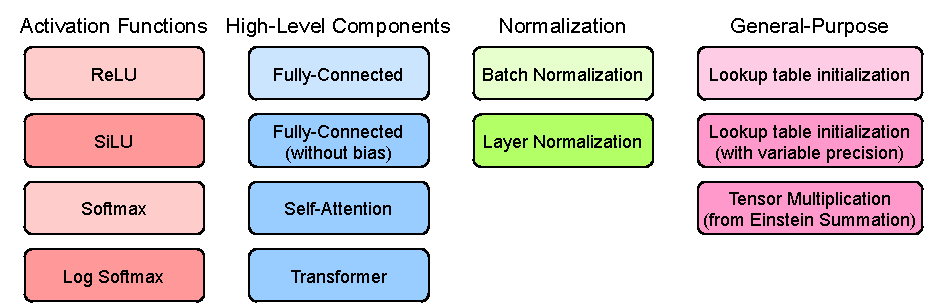
\includegraphics[trim={0cm 0cm 0cm 0cm}, clip, width=0.7\textwidth, center]{evaluation/hls4ml_blocks.pdf}
  \caption{Overview of the created implementations (dark-colored) and some existing components with similar functionality (light-colored).}
  \label{fig:hls4ml-contributions}
\end{figure}


\subsection{Activation Functions}
\indo{Mention SiLU which was experimented with}
\indo{Mention Log Softmax that implements the architecture from previous chapter}
\indo{|}
\indo{|}

\subsection{High-Level Components}
\indo{Briefly mention FC without bias as an optimization that saves initializing accumulators with bias values}
\indo{Talk in details about the C++ HLS challenges and achievements of self-attention and transformer}
\indo{|}
\indo{|}
\indo{|}
\indo{|}


\subsection{Normalization Layers}
\indo{Discuss how layer norm and batch norm actually differ}
\indo{|}
\indo{|}


\subsection{General-Purpose Blocks}
\indo{Explain the mechanism of function look up table initialization and how it was automatic}
\indo{|}
\indo{Show when automatic precision/range fails and how the new block addresses that by exposing int bit width as a parameter}
\indo{|}
\indo{|}
\indo{|}
\indo{Mention tensor einsum and the pragmas it uses}
\indo{|}

